%%%%%%%%%%%%%%%%%%%%%%%%%%%%%%%%%%%%%%%%%
% University/School Laboratory Report
% LaTeX Template
% Version 3.1 (25/3/14)
%
% This template has been downloaded from:
% http://www.LaTeXTemplates.com
%
% Original author:
% Linux and Unix Users Group at Virginia Tech Wiki 
% (https://vtluug.org/wiki/Example_LaTeX_chem_lab_report)
%
% License:
% CC BY-NC-SA 3.0 (http://creativecommons.org/licenses/by-nc-sa/3.0/)
%
%%%%%%%%%%%%%%%%%%%%%%%%%%%%%%%%%%%%%%%%%

%----------------------------------------------------------------------------------------
%	PACKAGES AND DOCUMENT CONFIGURATIONS
%----------------------------------------------------------------------------------------

\documentclass{article}

\usepackage[version=3]{mhchem} % Package for chemical equation typesetting
\usepackage{siunitx} % Provides the \SI{}{} and \si{} command for typesetting SI units
\usepackage{graphicx} % Required for the inclusion of images
\usepackage{natbib} % Required to change bibliography style to APA
\usepackage{amsmath} % Required for some math elements 
\usepackage{subfig}
\usepackage[final]{pdfpages}
\usepackage{float}
\usepackage{titlesec}
\usepackage[titletoc,toc,title]{appendix}
\usepackage{xfrac}

\newcommand{\itab}[1]{\hspace{0em}\rlap{#1}}
\newcommand{\tab}[1]{\hspace{.2\textwidth}\rlap{#1}}
\newcommand{\eq}[1]{\eqref{eq:#1}}
\newcommand{\fig}[1]{\ref{fig:#1}}
\newcommand{\te}[1]{\text{#1}}
\newcommand{\lahde}[2]{\cite[#2]{bib:#1}}
\setlength\parindent{0pt} % Removes all indentation from paragraphs

\renewcommand{\labelenumi}{\alph{enumi}.} % Make numbering in the enumerate environment by letter rather than number (e.g. section 6)

%\usepackage{times} % Uncomment to use the Times New Roman font

%----------------------------------------------------------------------------------------
%	DOCUMENT INFORMATION
%----------------------------------------------------------------------------------------

\title{JuroCalib\\ Energy calibration program for germanium array}
	
\date{\today} % Date for the report
\author{Joonas Ojala}

\begin{document}

\maketitle % Insert the title, author and date

% If you wish to include an abstract, uncomment the lines below
% \begin{abstract}
% Abstract text
% \end{abstract}

%----------------------------------------------------------------------------------------
%	SECTION 1
%----------------------------------------------------------------------------------------

\section{Foreword}
This energy calibration program has been done to help in energy calibration for germanium arrays at Accelerator laboratory of Jyväskylä. The program has been tested with data from of JUROGAMII , JUROGAMIII and conversion electrons from the Sage silicon detector with success!  


\section{Getting started}
JuroCalib run with Python3.6 including Numpy (Tested with 1.14.4) and Scipy (Tested with 1.1.0) packages. User need to install these packages! User can insert program folder in path of their desire. 
For example:\\
\textbf{ $\sim$/energyCalibration=$<$PATH$>$ }\\
The program folder has inside following folders:\\
\textbf{ -Source: } Contains program itself.This folder should contains following files files:energyCalibProgram.py, energyCalibration.py, gaussianFit.py, guiCommand.py, peakSearch.py, rawCalibration.py, readEnergies.py, readGUIFile.py,readOutput.py, readSettings.py.\\
\textbf{ -Input: } Default folder for input spectrum which user wants to calibrate.\\
\textbf{ -Output: } Default folder for output which are created by program.\\
\textbf{ -CalibrationFiles: } Contains files of peak energies which user want to use for calibration. The mixed source Eu-152 and Ba-133 is there as default (Euba.txt). One can find the format of calibration file from appendix  \ref{sec:appendices1}\\

\section{Starting  Calibration}
The easiest way to start the program goes as follows:\\
\textbf{ cd $<$PATH$>$/Source/ }\\
\textbf{ python3.6 energyCalibProgram.py }\\
This should open GUI (Graphical Unit Interface) of program which is shown in figure 
\begin{figure}
	\centering
	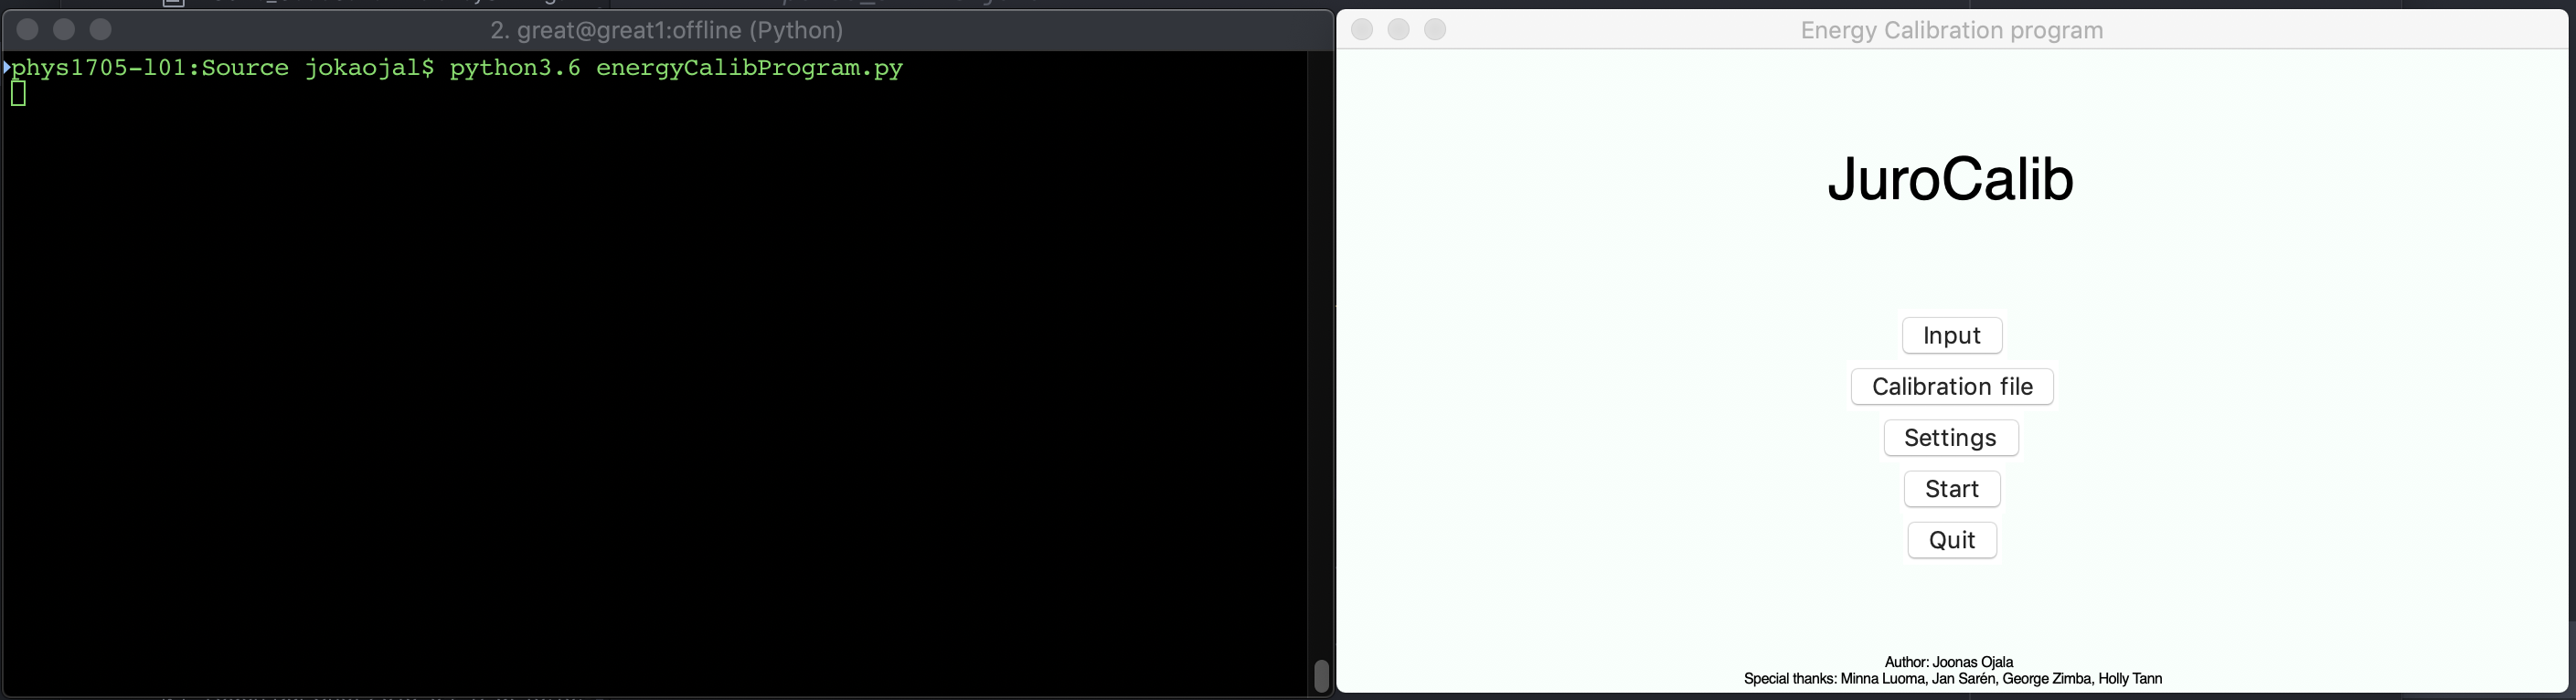
\includegraphics[width=1\linewidth]{GUI}
	\caption{One can see the commands to open GUI and GUI itself. Here one can see all the tabs which basically define the inputs before one can start calibration.}
	\label{fig:gui}
\end{figure}
Before starting the calibration, following objects need to be defined: location of input data, location of output folder location, calibration energy file (either location of user defined energy calibration file or default Eu-152 and Ba-133) and settings for peak search. In these instruction will follow  step by step, how to proceed to calibration.

\textbf{First} user defines the location of inputs and output folder.


\begin{appendices}

	\section{Eu-152 and Ba-133 calibration file}
	\label{sec:appendices1}
	\textit{\\
	$\#$Peaks on a table\\
	$\#$Peak energies unit in keV. If user want to use same energy difference in high and low energy,write the energy difference in Energy$\_$low
	$\#$Energy,Energy$\_$low(or Energy$\_$difference),(Energy$\_$high)\\
	$\#$The *-marked energies are used as a first selection in rawCalibration.py\\
	80.997,3\\
	121.7825,3,*\\
	244.6989,3\\
	276.398,3\\
	302.853,3\\
	344.281,3,2\\
	356.017,2,3\\
	383.851,3\\
	411.115,3\\
	443.965,3\\
	510.999,3\\
	778.903,3,*\\
	867.390,3\\
	964.055,3\\
	1112.087,3\\
	1408.022,3\\
}
\end{appendices}

\end{document}

%----------------------------------------------------------------------------------------
%	BIBLIOGRAPHY
%----------------------------------------------------------------------------------------

\bibliographystyle{unsrt}

\bibliography{sample}